\section{design}

\begin{figure}[t!]
 \centering
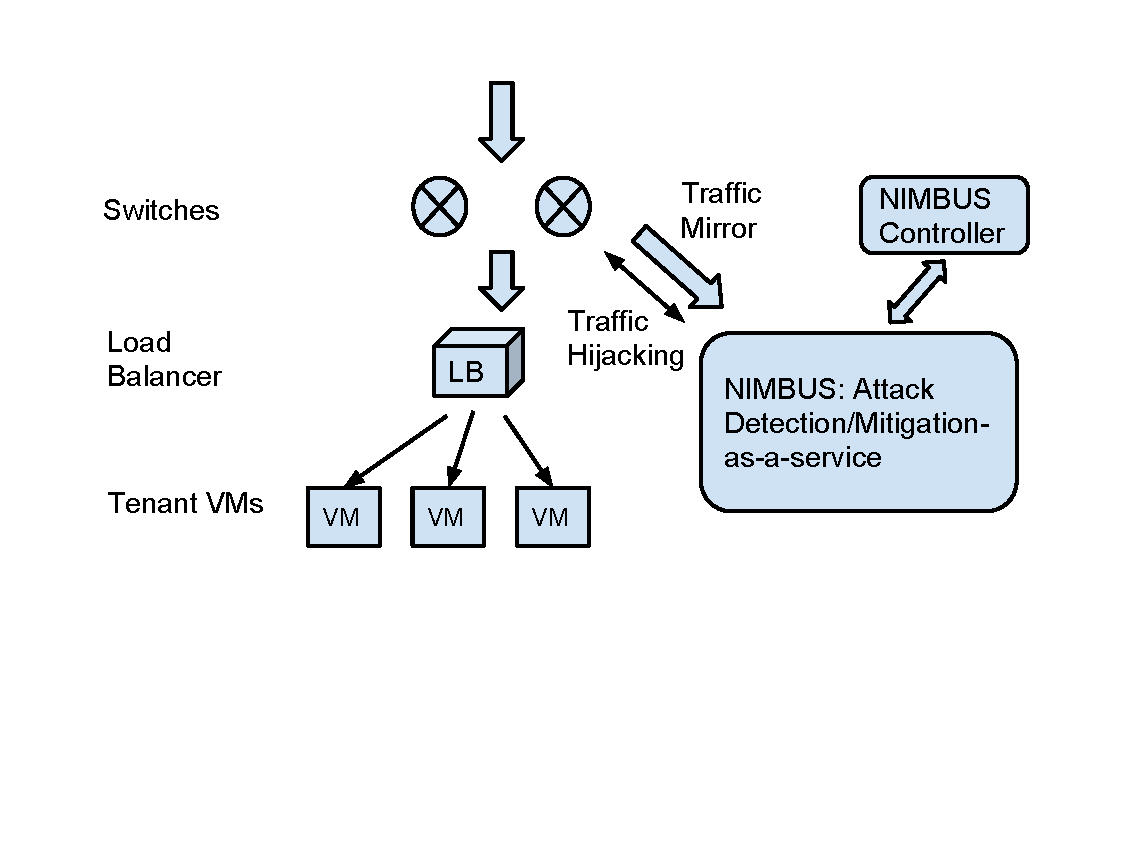
\includegraphics[width=\linewidth]{figs/scope.pdf}
\vspace{-0.82in}
\caption{\small Network scope of \nimbus deployment}
\vspace{-0.0in}
\label{fig:scope}
\end{figure}

\begin{figure}[t!]
 \centering
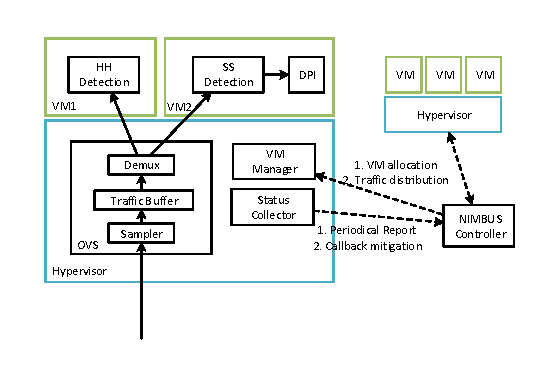
\includegraphics[width=\linewidth]{figs/arch.pdf}
\vspace{-0.22in}
\caption{\small \nimbus Architecture}
\vspace{-0.2in}
\label{fig:design}
\end{figure}


\nimbus can be deployed as either an in-band or an out-of-band
solution. The in-band solution requires faster scale-out to avoid affecting the data path and to ensure packet forwarding at line speed.
However, our prototype investigate the outband solution to avoid taking resources from the critical infrastructure (e.g., switches, software load balancers). 
As shown in Figure ~\ref{scope}, it requires the extra overhead of duplicating (e.g., port mirroring) the traffic to the detection and mitigation service. Further, as part of mitigation, \nimbus can also hijack a portion of traffic for scrubbing and send traffic back to network after dropping all attack traffic.

%\nimbus can be used for both inbound and outbound attacks. \minlan{anything more to say?}

%While \nimbus was designed to overcome limitations in commercial
%appliances, these can complement \nimbus nicely.  For example, we can
%leverage a scrubbing layer in switches to reduce the traffic to our
%service or use \nimbus to decide when to forward packets to
%hardware-based anomaly detection boxes for deep packet inspection.

We have designed \nimbus as a distributed architecture
(Figure~\ref{fig:design}) 
using an SDN-inspired framework, 
comprising a set of VM instances that analyze traffic for attack detection  
(called \emph{VMSentries}) and an \emph{auto-scale controller}
that (a) does scale-out/in of VM instances to avoid overloading,
(b) manages routing to traffic flows to them, and 
%(c) traffic sampling modules and 
(c) dynamically instantiates anomaly detector and mitigation modules on them.
%To enable applications and operators to flexibly specify their sampling, attack detection and mitigation strategies, 
%\nimbus exposes these functionalities through a RESTful API shown in Table~\ref{tab:autoscale-apidesign}. 

\parab{VMSentry.} The VMSentry is a pool of VMs instantiated on-demand for attack detection and mitigation. 
The role of a VMSentry is to passively collect ongoing traffic (e.g., via sampling), 
analyze it via detection modules, and prevent unauthorized traffic as configured by the SDN controller. 
The traffic is sampled in hypervisor and delivered to specific VM for analysis.
For each VMSentry, the control application 
would instantiate 
(1) a detector (e.g., heavy-hitter for TCP SYN/UDP floods, super-spreader for DNS reflection),
(2) configure the sampler in hypervisor for the new VM (e.g., sampling rate).
  %(2) attach a sampler (e.g., flow-based, packet-based, sample-and-hold) and set its configurable sampling rate, 
%(3) provide a callback URI, and 
(3) then install it on that VM. 
When the detector instances detect an on-going attack, they invoke a callback to controller. The controller can then decide to 
specify a mitigation strategy in an application-specific manner. 
For instance, it can set up rules for access control, rate-limit or redirect 
anomalous traffic (not the copy) to \nimbus devices for scrubbing or an in-depth analysis. 
Setting up mitigator instances is similar to that of detectors with a specific mitigator action (e.g., redirect, scrub, mirror, allow, deny) .
%and %optionally 
%specify the flow (either through a standard 5-tuple or $<$VIP, protocol$>$ pair) along with a callback URI.

Our implementation of \nimbus 
separates mechanism from policy by partitioning VMSentry functionalities between the hypervisorl and VM: 
packet sampling is done at the hypervisor for performance and efficiency, 
%hypervisor layer for performance and efficiency, 
%(reduce the number of packets sent to the user space) 
and the 
detection and mitigation policies reside in the VM's user space to ensure flexibility and adaption at run-time.
This separation allows 
multi-stage attack detection and mitigation e.g.,  traffic from source IPs sending a TCP SYN attack can be forwarded for deep packet inspection.
The intuition behind co-locating detectors and mitigators on the same VM instance 
is that it reduces the critical overheads of  
traffic redirection, which can be significant~\cite{Sylvia2011}, and leverages the caches to store the packet content. Further, this approach  
avoids the controller overheads 
of managing different types of VMSentries. 
%that gets called when the mitigator detects the termination of an on-going attack. 

Given limited computing and memory capacity in VM instances, a key question is what granularity to use to uniquely identify 
and specify actions on anomalous flows. %Specifically, 
While using the five-tuple flow identifier allows flexibility to specify detection and mitigation at a fine granularity,  
it risks high resource overheads, 
missing attacks at the aggregate level (e.g., VIP) or treating correlated attacks as independent ones. 
In the cloud setup, since traffic flows can be logically partitioned by VIPs, \nimbus addresses flows using $<$VIP, protocol$>$ pairs. This allows us to 
(a) efficiently manage state for a large number of flows at each VMSentry,
and (b) design customized attack detection solutions for individual VIPs;
we leave the investigation of flow identifiers at finer granularities for future work.
Note that the traffic flows for a $<$VIP, protocol$>$ pair can
be spread across VM instances 
similar in spirit to SLB~\cite{Patel13}. 
%akin to SLB~\cite{Patel13}.  
%\navendu{DO YOU MEAN "we allocate one  $<$VIP, protocol$>$" OR "detector+mitigator" to the same VM.} \minlan{one  $<$VIP, protocol$>$} \navendu{minlan: I'm not clear how to weave in this argument (vip,prot) split across vms like in slb (using ECMP; all SLBs have identical VIP to DIP mapping) or keep to a single one 
%\navendu{Rui: anything else to add?} 
	
% \delete{
% 	As our measurement results show, different protocols are vulnerable for different types of attacks. For example, RDP traffic are usually under spread-based attacks while TCP traffic are more vulnerable to volume based attacks. 
% The management decisions on VIP and protocol fields only can guarantee the scalability of our system. (Note that SLB also made load balancing decisions on VIPs to ensure scalability.)
% However, we choose not to use finer granularities (e.g., five tuple flows) to reduce the overhead of managing the system. 

% There are two ways of using the VMs when each $<$VIP, protocol$>$ needs a pipeline of detection and mitigation solutions. First, we can use each VM to run one function (e.g., heavy hitter detection) but then redirect traffic to different VMs for different functions. Second, we can use one VM to perform all the attack detection/mitigation solutions for the same $<$VIP, protocol$>$. 
% }


\parab{SDN auto-scale controller.} 
The controller collects the load information across instances every 
measurement interval. 
If needed, it computes a new allocation of traffic distribution across existing VMs and
scale-out/in VM instances. Finally, it installs routing rules to redirect the traffic. 


%\parae{Traffic splitting to VMs:} 
In the cloud environment, the traffic patterns destined to a VMSentry may quickly increase due to higher traffic rate of 
existing flows (e.g., volume-based attacks) or setup of new flows (e.g., due to tenant deployment). Thus, a 
key requirement is to avoid overload of VMSentry instances as it risks impacting accuracy and effectiveness of attack detection and mitigation. 
To address this issue, the controller monitors load at each instance
and dynamically re-allocates traffic across the existing and possibly newly-instantiated VMs. 
To implement this functionality, however,  
we need to make three design decisions: 
(1) What metric to use to measure load? 
(2) How to redistribute traffic across instances? and 
(3) Do we need to transfer flow state from an overloaded instance to a new/existing one? 

First, we choose to use CPU as the VM load metric because our experiments show that CPU utilization is strongly correlated to traffic rate. 
%he packet sampling at the kernel and the packet inspection at the user space are two potential bottlenecks and both are bottlenecked by their CPU usage. We can also extend this to other metrics such as memory and bandwidth usage. 
We model CPU usage as a function of the traffic volume for different anomaly detection/mitigation algorithms to set the maximum and minimum load threshold. 

Second, to redistribute traffic, we formulate a bin-packing problem which takes the top-k $<$VIP, protocol$>$ tuples by traffic rate as input from the overloaded
VMs and uses the first-fit decreasing algorithm that allocates traffic to the 
other VMs while minimizing the migrated traffic. If the problem is infeasible,
it allocates new VMSentry instances so that no instance is overloaded. Similarly, for scale-in, all VMs whose load falls below the minimum threshold become 
candidates for standby or being shut down. The VMs selected to be taken out of operation stop accepting new flows and transition to inactive state once incoming traffic ceases. Note that other traffic redistribution and auto-scaling approaches can be applied in our framework.   
We observe that many attack detection/mitigations tasks are state independent. For example, to detect the heavy hitters of traffic to a VIP, we typically need to keep track of the traffic volumes only in the 
most recent intervals. This simplifies traffic redistribution as we do not need to transfer potentially large measurement state of transitioned flows.
For those measurement tasks that do need state transitions, we can 
add a constraint for the traffic distribution algorithm 
to avoid moving their traffic. 

Third, to redistribute traffic, the controller changes routing entries at the upstream switches/routers to redirect traffic. 
Finally, to quickly transition the service to a stable state during churn, \nimbus maintains a standby resource pool of VMs which
are in active mode and can take the load immediately.
%hich have much shorter restart times compared to loading and deploying new VM images from disk;
We show the efficacy of this approach in next section.



